\documentclass[12pt]{article}
\usepackage[pdfborder={0 0 0.5 [3 2]}, plainpages=false]{hyperref}%
\usepackage[left=1in,right=1in,top=1in,bottom=1in]{geometry}%
\usepackage[shortalphabetic]{amsrefs}%
\usepackage{amsmath}
\usepackage{enumerate}
% \usepackage{enumitem}
\usepackage{amssymb}                
\usepackage{amsmath}                
\usepackage{amsfonts}
\usepackage{amsthm}
\usepackage{bbm}
\usepackage[table,xcdraw]{xcolor}
\usepackage{tikz}
\usepackage{float}
\usepackage{booktabs}
\usepackage{svg}
\usepackage{mathtools}
\usepackage{cool}
\usepackage{url}
\usepackage{graphicx,epsfig}
\usepackage{makecell}
\usepackage{array}

\def\noi{\noindent}
\def\T{{\mathbb T}}
\def\R{{\mathbb R}}
\def\N{{\mathbb N}}
\def\C{{\mathbb C}}
\def\Z{{\mathbb Z}}
\def\P{{\mathbb P}}
\def\E{{\mathbb E}}
\def\Q{\mathbb{Q}}
\def\ind{{\mathbb I}}

\DeclareMathOperator{\spn}{span}
\DeclareMathOperator{\ran}{range}

\setlength\parindent{0pt}

\graphicspath{ {suspension/} }

\newtheorem{lemma}{Lemma}
\newtheorem{theorem}{Theorem}
\newtheorem{corollary}{Corollary}
\newtheorem{definition}{Definition}
\newtheorem{proposition}{Proposition}
\newtheorem{assumption}{Assumption}
\newtheorem{hypothesis}{Hypothesis}

\newtheorem{notation}{Notation}

\begin{document}

\section{Chen-McKenna Suspension Bridge Equation}

\subsection{Background}

In \cite{McKenna1990}, McKenna and Walter propose the following equation to model traveling waves on an infinitely long suspended beam

\begin{equation}\label{susp}
u_{tt} + u_{xxxx} + u^+ - 1 = 0,
\end{equation}

where $u^+ = \max(u, 0)$. This model was motivated by observations of traveling waves on suspension bridges. In \cite{Chen1997}, Chen and McKenna introduce the following smooth approximation to \eqref{susp}

\begin{equation}\label{susp2}
u_{tt} + u_{xxxx} + e^{u-1} - 1 = 0.
\end{equation}

The analytic function $e^{u-1}$ is less likely to introduce error into numerical schemes than the non-smooth function $u^+$. Making the change of variables $u - 1 \mapsto u$ in \eqref{susp2} so that localized solutions will decay to a baseline of 0, we will consider the equation

\begin{equation}\label{susp3}
u_{tt} + u_{xxxx} + e^{u} - 1 = 0.
\end{equation}

Writing this in a co-moving frame with speed $c$ by letting $\xi = x - ct$, equation \eqref{susp3} becomes

\begin{equation}\label{suspc}
u_{tt} - 2 c u_{x t} + u_{xxxx} + c^2 u_{xx} + e^{u} - 1 = 0,
\end{equation}

where we have renamed the independent variable back to $x$. An equilibrium solution to \eqref{suspc} satisfies the ODE

\begin{equation}\label{eqODE}
u_{xxxx} + c^2 u_{xx} + e^{u} - 1 = 0.
\end{equation}

In \cite[Theorem 11]{Smets2002}, Smets and van den Berg prove existence of a localized, symmetric solution $q(x; c)$ to \eqref{eqODE} for almost all speeds $c \in (0, \sqrt{2})$. In \cite[Theorem 1]{Berg2018}, van den Berg et al use a computer-assisted proof technique to show existence of such solutions to \eqref{eqODE} for all speeds $c$ with $c^2 \in [0.5, 1.9]$. For what follows, we will take $c \in [\sqrt{0.5}, \sqrt{1.9}]$ so that a primary pulse solution $q(x; c)$ is known to exist. \\

We are interested in the existence and stability of multi-pulse equilibrium solutions to \eqref{suspc}. A multi-pulse is a localized, multi-modal solution $q_n(x; c) $to \eqref{eqODE} which resembles multiple, well-separated copies of the primary pulse $q(x; c)$. First, we look at existence. For any solution $u_*$ to \eqref{eqODE}, the linearization of \eqref{eqODE} about $u_*$ is given by

\begin{equation}\label{defA0}
A_0(u^*) = \partial_x^4 + c^2 \partial_x^2 + e^{u_*}.
\end{equation}

For $c \in (0, \sqrt{2})$, $A_0(0)$ is hyperbolic, and its spectrum is

\begin{align}\label{specA00}
\sigma(A_0(0)) &= \pm \sqrt{\frac{-c^2 \pm \sqrt{c^4 - 4}}{2} } = \pm \alpha \pm \beta i,
\end{align}

for some $\alpha, \beta > 0$. The constant $\alpha$ is the exponential decay rate of localized solutions to \eqref{eqODE}. We make the following hypothesis.

\begin{hypothesis}\label{A0kernel}
The operator $A_0(q(x; c))$ on $L^2(\R)$ has a one-dimensional kernel spanned by $\partial_x q(x; c)$.
\end{hypothesis}

From this hypothesis, it follows that the primary pulse $q(x; c)$ is transversely constructed. Thus we have the following theorem, which is adapted from \cite[Theorem 3.6]{Sandstede1997}.

\begin{theorem}\label{multiexist}
Let $q(x; c)$ be a localized solution to \eqref{eqODE} for which Hypothesis \ref{A0kernel} holds. Then for any $n \geq 2$ and any sequence of nonnegative integers $k_1, \dots, k_{n-1}$ with at least one of the $k_j \in \{0, 1 \}$, there exists a nonnegative integer $m_0$ and $\delta > 0$ such that
\begin{enumerate}[(i)]
	\item For any integer $m$ with $m \geq m_0$, there exists a unique $n-$modal solution $q_n(x, c)$ to \eqref{eqODE} which is of the form
	\begin{align}\label{qn}
	q_n(x; c) = \sum_{j = 1}^{n} q^j(x; c) + r(x; c),
	\end{align}
	where each $q^j(x; c)$ is a translate of the primary pulse $q(x; c)$. The distance between the peaks of $q^j$ and $q^{j+1}$ is $2 X_j$, where
	\begin{equation*}
	X_j \approx \frac{\pi}{\beta}(2 m + k_j) + \tilde{X},
	\end{equation*}
	$\beta$ is defined in \eqref{specA00}, and $\tilde{X}$ is a constant. The remainder term $r(x; c)$ satisfies
	\begin{equation}\label{rbound}
	||r|| \leq C e^{-\alpha X_m},
	\end{equation}
	where $\alpha$ is defined in \eqref{specA00} and $X_m = \min\{X_1, \dots, X_{n-1}\}$.

	\item The linear operator $A_0(q_n)$ on $L^2(\R)$ has precisely $n$ real eigenvalues $\nu_j$ with $|\nu_j| < \delta$, where $\nu_n = 0$ is a simple eigenvalue and for $j = 1, \dots, n-1$,
	\begin{align*}
	\nu_j < 0 \text{ if } k_j \text{ is odd} \\
	\nu_j > 0 \text{ if } k_j \text{ is even} 
	\end{align*}

	\item For $j = 1, \dots, n-1$, $\nu_j = \mathcal{O}(e^{-2\alpha X_m})$ and the eigenfunctions $s_j$ are given by
	\begin{align}\label{sj}
	s_j = \sum_{i = 1}^{n} d_{ji} q^i_x + w_j
	\end{align}
	where $d_{ji} \in \C$ are constants and the remainder terms $w_j$ satisfy
	\begin{equation}\label{sjwbound}
	||w_j|| \leq C e^{-2 \alpha X_m}
	\end{equation}

\end{enumerate}

\begin{proof}
Equation \eqref{eqODE} is Hamiltonian with energy

\begin{equation}\label{defH}
H(u) = u_x u_{xxx} - \frac{1}{2}u_{xx}^2 + \frac{c^2}{2}u_x^2 + e^u - u.
\end{equation}

Using \eqref{specA00}, \eqref{defH}, Hypothesis \ref{A0kernel}, and the fact that the Melnikov integral $M = \int_{-\infty}^\infty |q_x|^2 dx$ is positive, (i) and (ii) follow from Theorem 3.6 in \cite{Sandstede1997}, except for the bound on $r(x; c)$ in (i), which follows from \cite{Sanstede1993} and \cite{Sandstede1998}. The eigenvalues $\nu_j$ are real since $A_0(q_n)$ is self-adjoint. Part (iii) follows from \cite{Sandstede1998}.
\end{proof}
\end{theorem}

To determine linear PDE stability of these multi-pulse solutions, we look at the linearization of the PDE \eqref{suspc} about $q_n(x; c)$, which is the following quadratic eigenvalue problem

\begin{equation}\label{quadeig}
P_2(\lambda; q_n)v =  [A_2 \lambda^2 + A_1 \lambda + A_0(q_n)]v = 0,
\end{equation}

where $A_0(q_n)$ is defined in \eqref{defA0} and 

\begin{align}
A_1 &= -2 c \partial_x \\
A_2 &= I
\end{align}

For $c \in (0, \sqrt{2})$, by the Weyl essential spectrum theorem, the essential spectrum of \eqref{quadeig} is independent of $q_n$ and is given by

\begin{equation}\label{quadess}
\sigma_{\text{ess}}(P_2) = (-\infty, \rho] \cup [\rho, \infty),
\end{equation}

where $\rho > 0$ and is the minimum of the function $\lambda(r) = c r + \sqrt{1 + r^4}$; this minimum is positive for $c \in (0, \sqrt{2})$. Thus the essential spectrum is purely imaginary and bounded away from 0.\\

Linear PDE stability thus depends on the point spectrum. We will use the Krein matrix to find the eigenvalues of \eqref{quadeig}. Applying Theorem \ref{multiexist}, let $\{\nu_1, \dots, \nu_n\}$ be the small eigenvalues of $A_0(q_n)$, and let \{$s_1, \dots, s_n\}$ be the corresponding eigenfunctions. Define the space $S$ by

\begin{equation}\label{defS}
S = \spn\{s_1, \dots, s_n \},
\end{equation}

and define the Krein matrix $K_S(z)$ as on P.4 OF THIS PAPER. We make the following hypotheses, which, by \cite[Theorems 5.5 and 3]{Grillakis1987}, give stability of the primary pulse $q(x; c)$.

\begin{hypothesis}\label{PDEexisthyp}
For every initial condition $u_0(x)$ there exists a solution $u(x, t)$ to \eqref{suspc} on the interval $I = [0, T]$, where $T$ only depends on $\max{ \{ ||u_0||, ||(u_0)_t|| \} }$.
\end{hypothesis}

\begin{hypothesis}\label{A0neg}
The operator $A_0(q)$ has a unique, simple negative eigenvalue $\lambda_- < 0$ with corresponding eigenfunction $v_-(x)$.
\end{hypothesis}

\begin{hypothesis}\label{dccpos}
$d''(c) > 0$ for $c^2 \in (0, 2)$, where $d(c)$ is defined in \cite[Equation (2.16)]{Grillakis1987} and 

\begin{equation}\label{dcc}
d''(c) = -\frac{\partial}{\partial c} \left( c ||q_x||^2 \right).
\end{equation}
\end{hypothesis}

We now present the following theorem, which is the main result of this section.

\begin{theorem}\label{Kreindiag}
Let $q_n(x; c)$ be an $n-$modal solution to \eqref{eqODE}. Let $\nu_1, \dots, \nu_n$ be the small eigenvalues of $A_0(q_n)$, as defined in Theorem \ref{multiexist}. Assume Hypotheses \ref{A0kernel}, \ref{PDEexisthyp}, \ref{A0neg}, and \ref{dccpos}. Then the Krein matrix is given by

\begin{equation}\label{Kreinapprox}
K_S(z) = ||q_x||^2 \text{diag} (\nu_1, \dots, \nu_n)
 + d''(c) I \overline{z}^2 + \mathcal{O}(e^{-(3 \alpha/2) X_m}|z| + |z|^3),
\end{equation}

which is diagonal to leading order.

\end{theorem}

As a corollary, we have the following criteria for linear PDE stability and instability of the multi-pulse solutions $q_n(x; c)$.

\begin{corollary}\label{stabcrit}
Let $q_n(x; c)$ be an $n-$pulse solution to \eqref{eqODE}, constructed as in Theorem \ref{multiexist} using the sequence of nonnegative integers $\{ k_1, \dots, k_{n-1} \}$. Assume the same hypotheses as in Theorem \ref{Kreindiag}. Let $\nu_1, \dots, \nu_n$ be the small eigenvalues of $A_0(q_n)$, where $\nu_n = 0$.
\begin{enumerate}[(i)]
	\item If $\nu_1, \dots, \nu_{n-1} < 0$ (equivalently, all $k_j$ are odd), then \eqref{quadeig} has $2n - 2$ purely imaginary eigenvalues near 0, which are given by

	\begin{equation}\label{npulseKreineigs}
	\lambda_j^\pm = \pm i \left( ||q_x|| \sqrt{ \frac{|\nu_j|}{d''(c)} } + \mathcal{O}(e^{-(3 \alpha/2) X_m}) \right).
	\end{equation}

	Thus $q_n(x; c)$ is linearly neutrally stable.

	\item If $\nu_j > 0$ for some $j = 1, \dots, n-1$ (equivalently, at least one $k_j$ is even), then \eqref{quadeig} has at least one eigenvalue with positive real part. Thus $q_n(x; c)$ is linearly unstable.
\end{enumerate}

\end{corollary}

\subsection{Numerics}

In this section, we show numerical results to illustrate the results of the previous section. First, we can construct a primary pulse solution $q(x; c)$ numerically using the string method from \cite{Chamard2011}. Figure \ref{fig:single1} shows these solutions for the same values of $c$ as in \cite[Figure 3]{Chen1997}.

\begin{figure}[H]
\centering
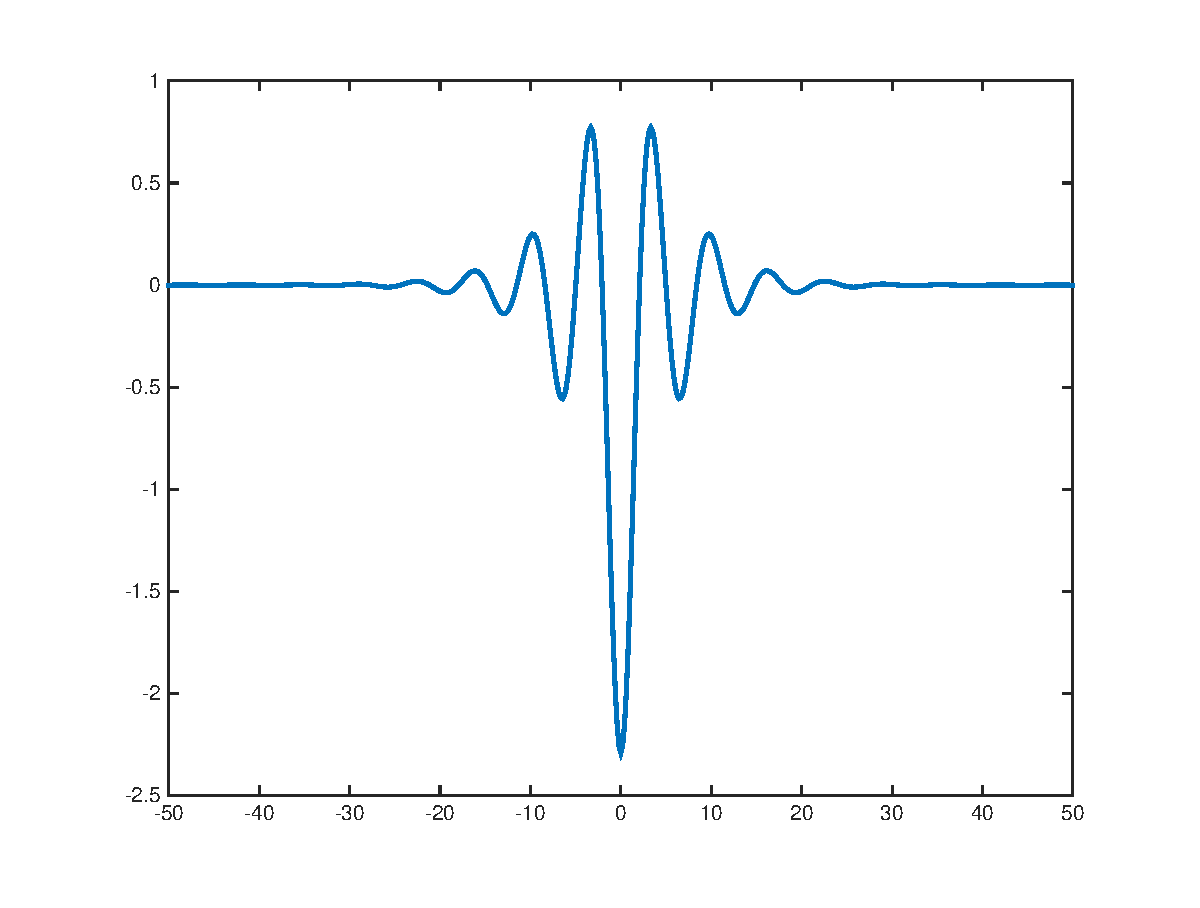
\includegraphics[width=8cm]{single1354.eps}
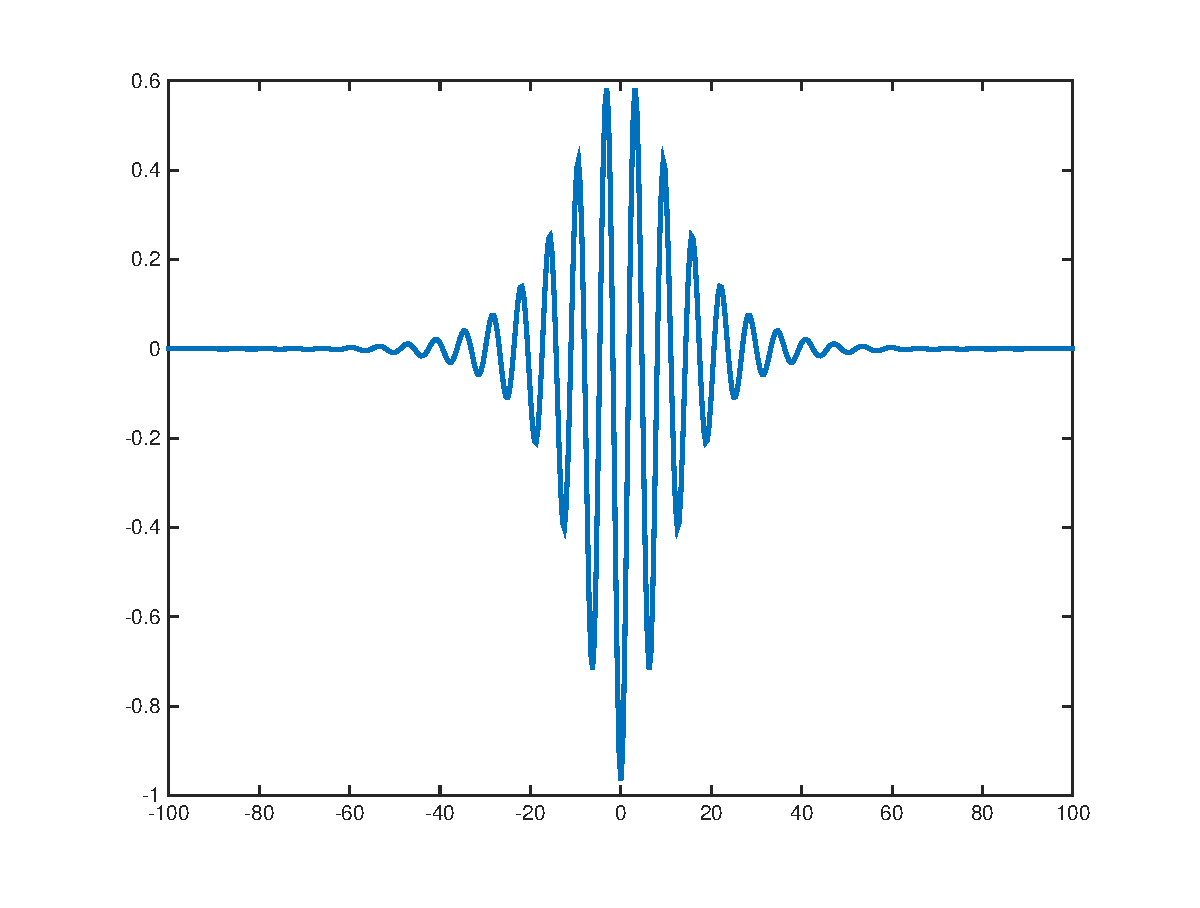
\includegraphics[width=8cm]{single14.eps}
\caption{Primary pulse solutions $q(x;c)$ to \eqref{eqODE} for $c = 1.354$ (left) and $c = 1.40$ (right). Finite difference methods, $N = 512$.}
\label{fig:single1}
\end{figure}

Next, we compute the spectrum of the operator $A_0(q(x; c))$ numerically using Matlab's \texttt{eig} function. In Figure \ref{fig:specA0}, we note the presence of a simple eigenvalue at 0 and a simple negative eigenvalue, which support Hypotheses \ref{A0kernel} and \ref{A0neg}; we also see that the essential spectrum is positive and bounded away from 0.

\begin{figure}[H]
\centering
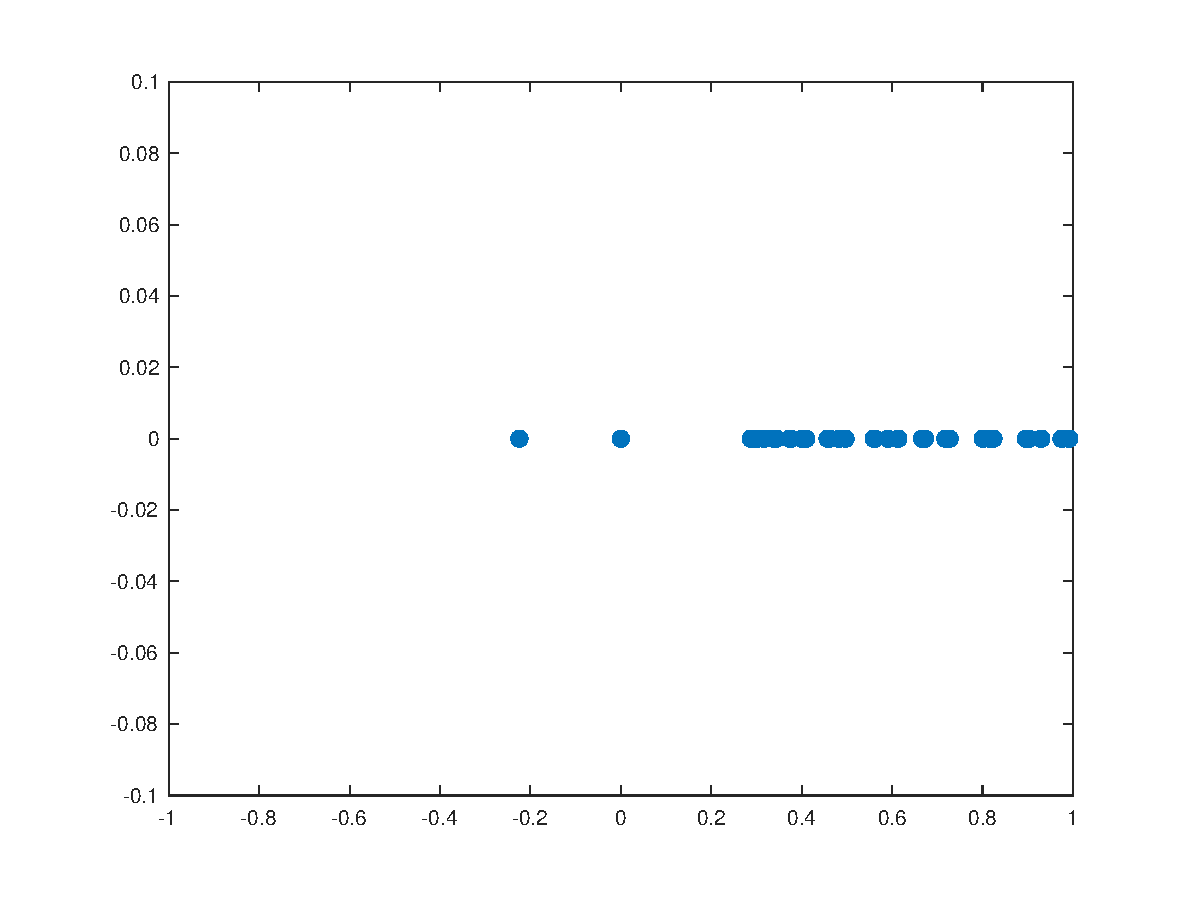
\includegraphics[width=8cm]{specA0.eps}
\caption{Spectrum of $A_0(q(x; c))$, the linearization of \eqref{eqODE} about a single pulse $q(x;c)$. $c = 1.3$. Finite difference methods, $N = 513$.}
\label{fig:specA0}
\end{figure}

We can construct multi-pulse solutions numerically by joining together multiple copies of the primary pulse and using Matlab's \texttt{fsolve} function; consecutive distances between peaks given by Theorem \ref{multiexist}. The first four double pulse solutions are shown in Figure \ref{fig:double}.

\begin{figure}[H]
\centering
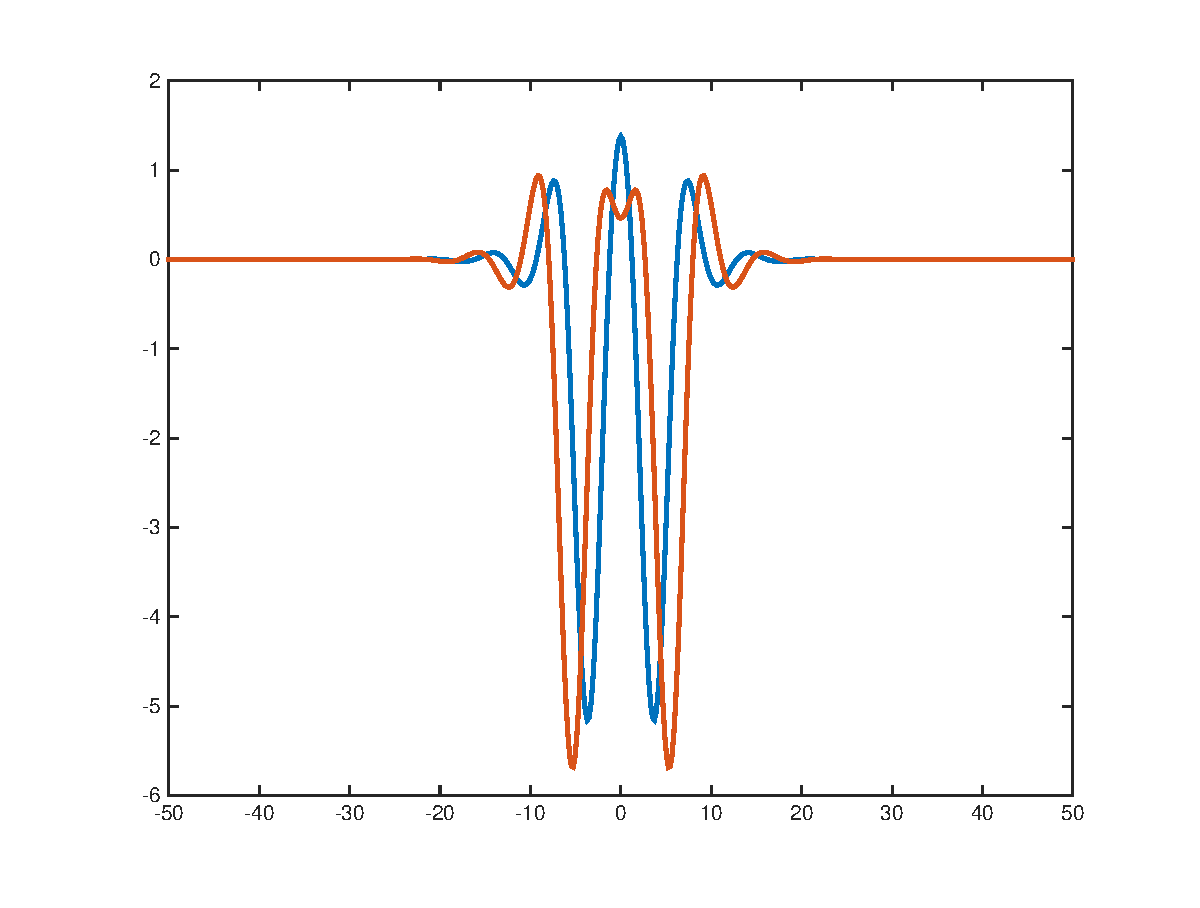
\includegraphics[width=8cm]{double12_12.eps}
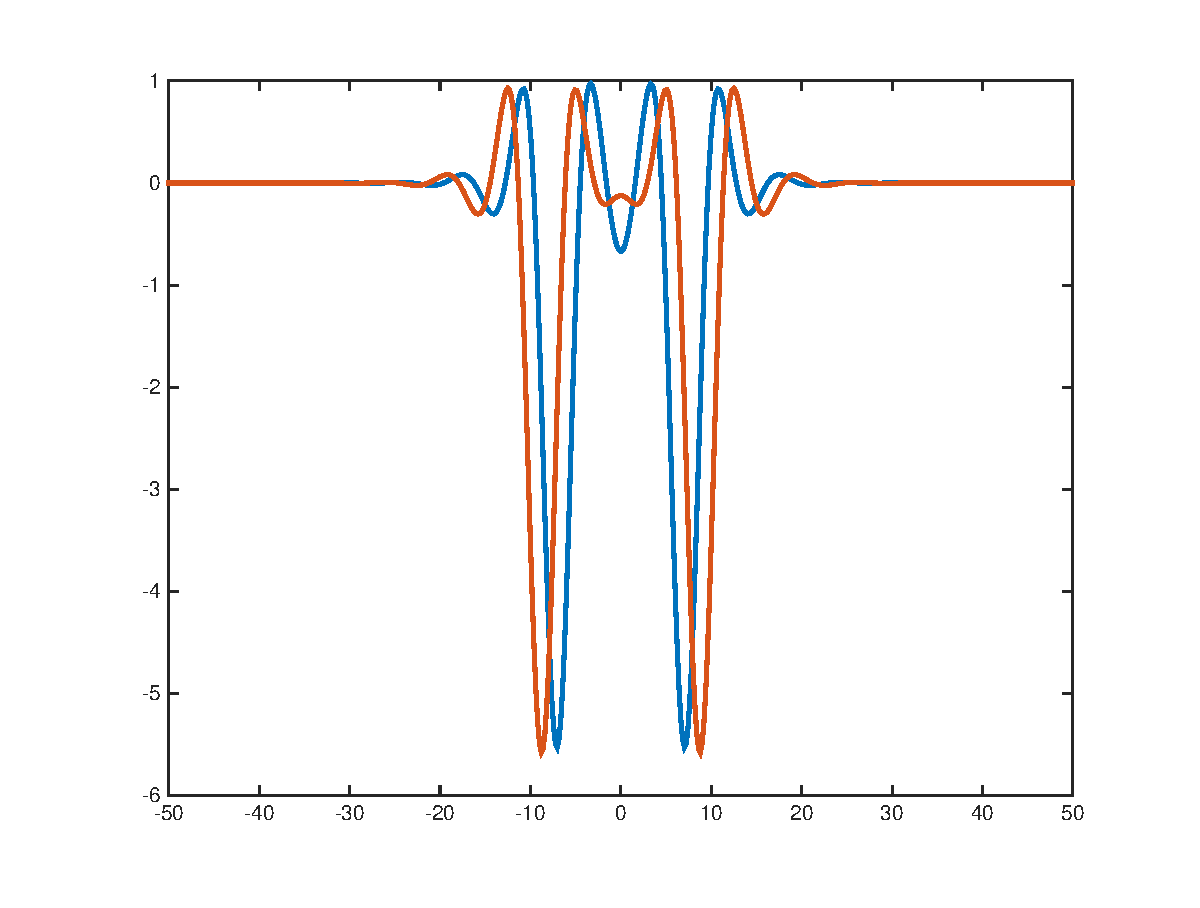
\includegraphics[width=8cm]{double12_34.eps}
\caption{Double pulse solutions $q_2(x; c)$ to \eqref{eqODE} for $c = 1.2$. Double pulses 0 and 1 (left). Double pulses 2 and 3 (right).}
\label{fig:double}
\end{figure}

We can verify part (ii) of Theorem \ref{multiexist} numerically by computing the spectrum of $A_0(q_2(x; c))$. The spectrum of $A_0(q_2)$ for double pulses 0 and 1 are shown in Figure \ref{fig:specA0double}. In both cases, there is an eigenvalue at 0. For double pulse 0, there is an additional positive eigenvalue, and for double pulse 1, there is an additional negative eigenvalue.

\begin{figure}[H]
\centering
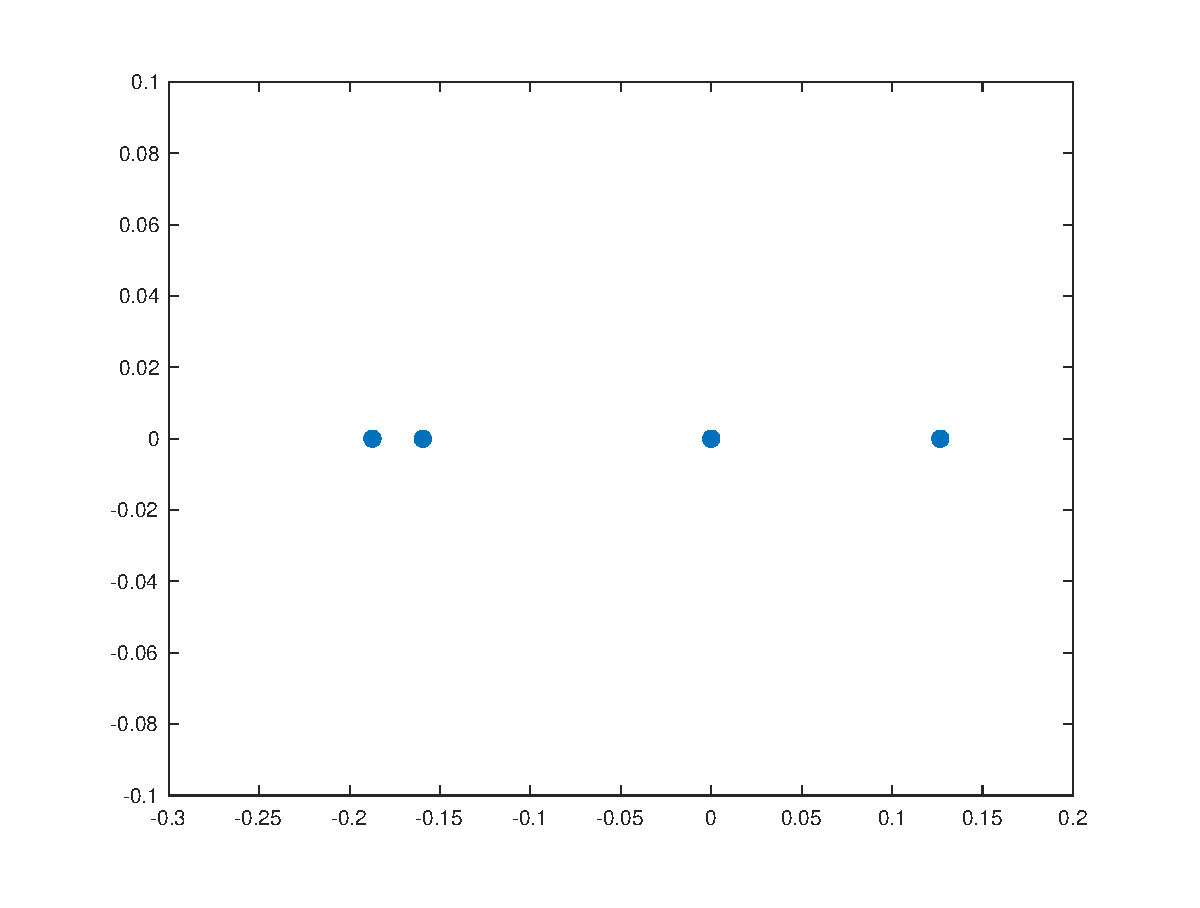
\includegraphics[width=8cm]{specA0d1}
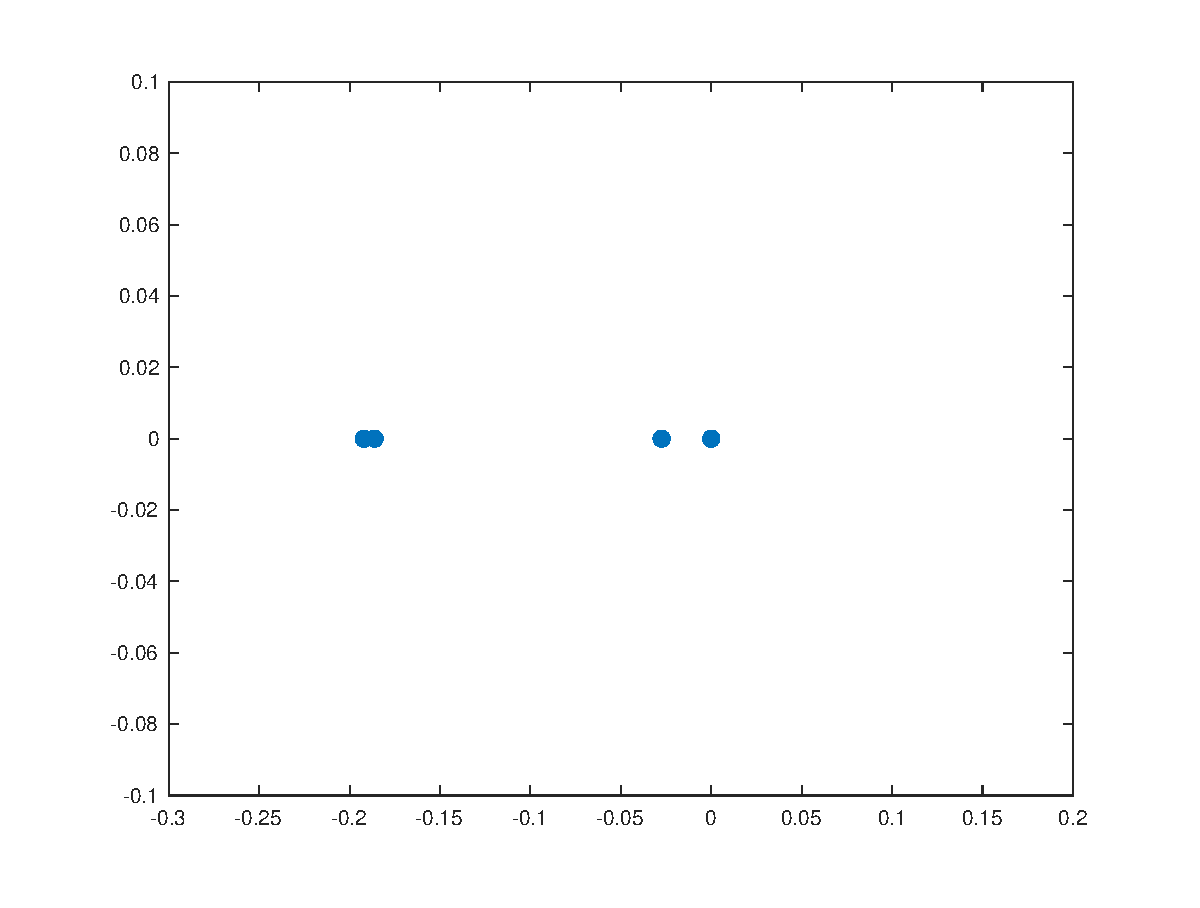
\includegraphics[width=8cm]{specA0d2}
\caption{Eigenvalues of $A_0(q_2)$ for $c = 1.2$. Double pulses 0 (left) and 1 (right).}
\label{fig:specA0double}
\end{figure}

Finally, we verify Corollary \ref{stabcrit} by computing the eigenvalues of \eqref{quadeig} directly using the Matlab package \texttt{quadeig} from \cite{Hammarling2013}. For double pulse 0, $A_0(q_2)$ has one small positive eigenvalue, thus, by Corollary \ref{stabcrit}, equation \eqref{quadeig} has an eigenvalue with positive real part. For double pulse 1, the small eigenvalue of $A_0(q_2)$ is negative, thus by Corollary \ref{stabcrit}, the eigenvalues of \eqref{quadeig} are purely imaginary. These are shown in Figure \ref{fig:quadeigdouble}.

\begin{figure}[H]
\centering
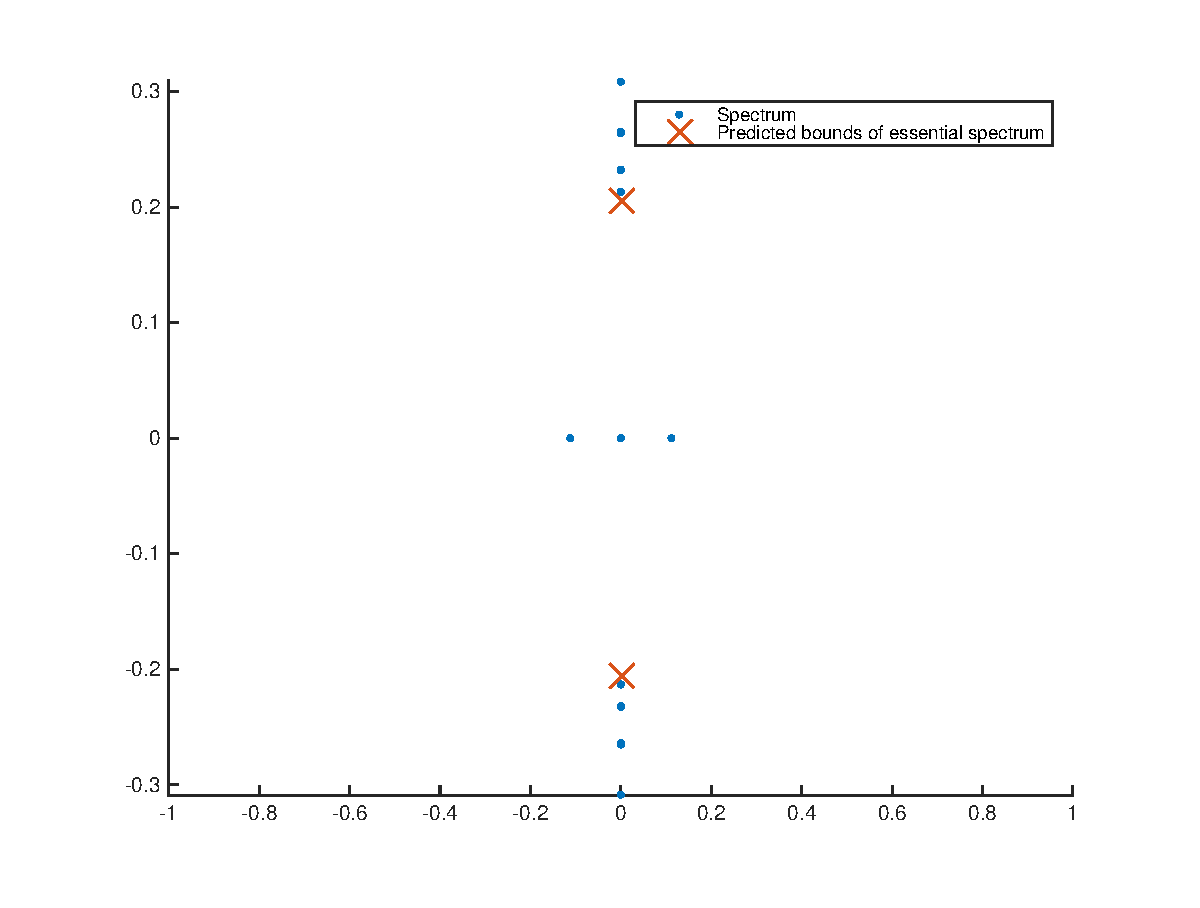
\includegraphics[width=8cm]{spec12_double1.eps}
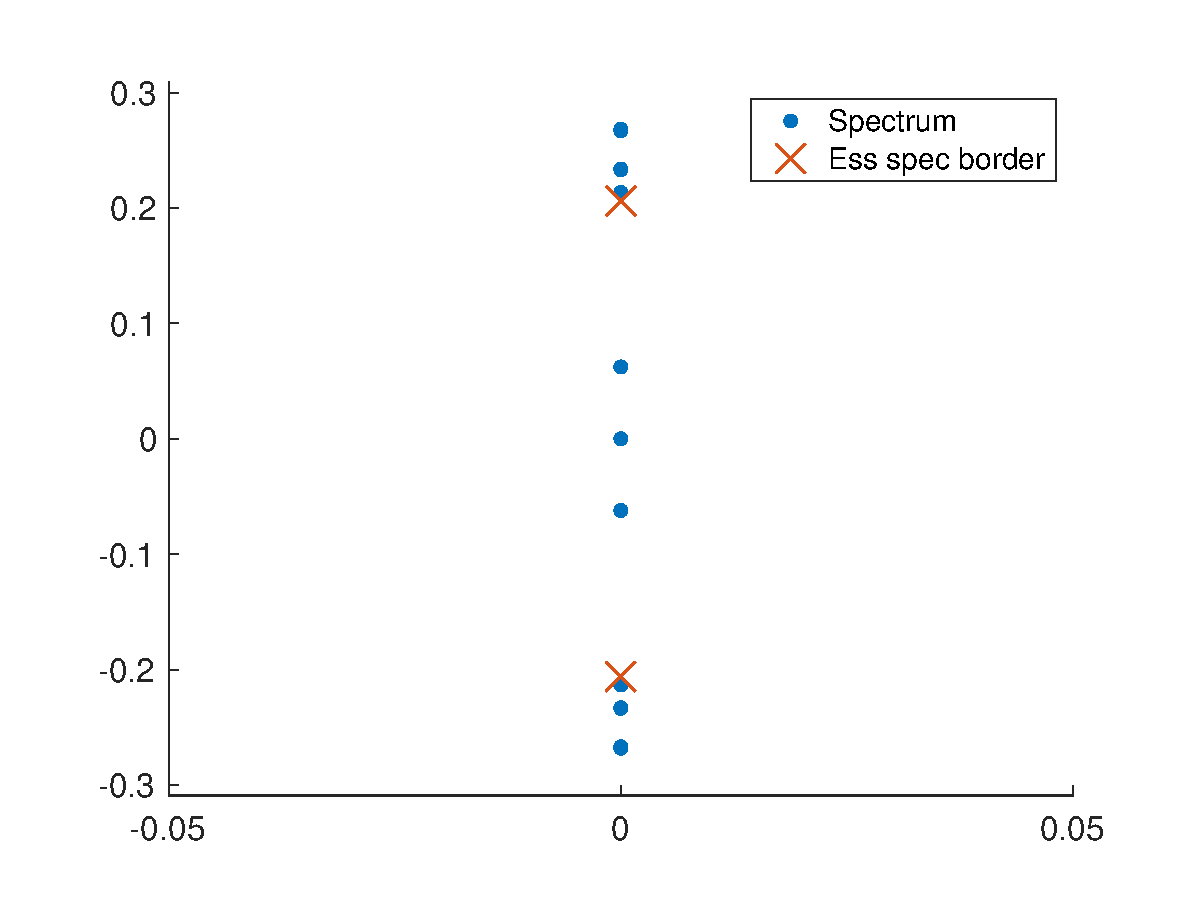
\includegraphics[width=8cm]{spec12_double2.eps}
\caption{Spectrum of \eqref{quadeig} for double pulses 0 (left) and 1 (right). Finite difference methods, $N = 512$, $c = 1.2$.}
\label{fig:quadeigdouble}
\end{figure}

WHAT TO DO WITH KREIN COLLISION?\\

For other values of $c$, the odd-numbered double pulses have the same eigenvalue pattern, so we will focus on the even-numbered double pulses. Let's look at $c = 1.354$ (this value was used in \cite{Chen1997}). For Double Pulse 2, we now have a quartet of interaction eigenvalues. Their imaginary part now lies \emph{outside} the essential spectrum gap. This suggests that a Krein collision has occurred, where the interaction eigenvalues collide with the smallest essential spectrum eigenvalue and then form a quartet.

\begin{figure}[H]
\centering
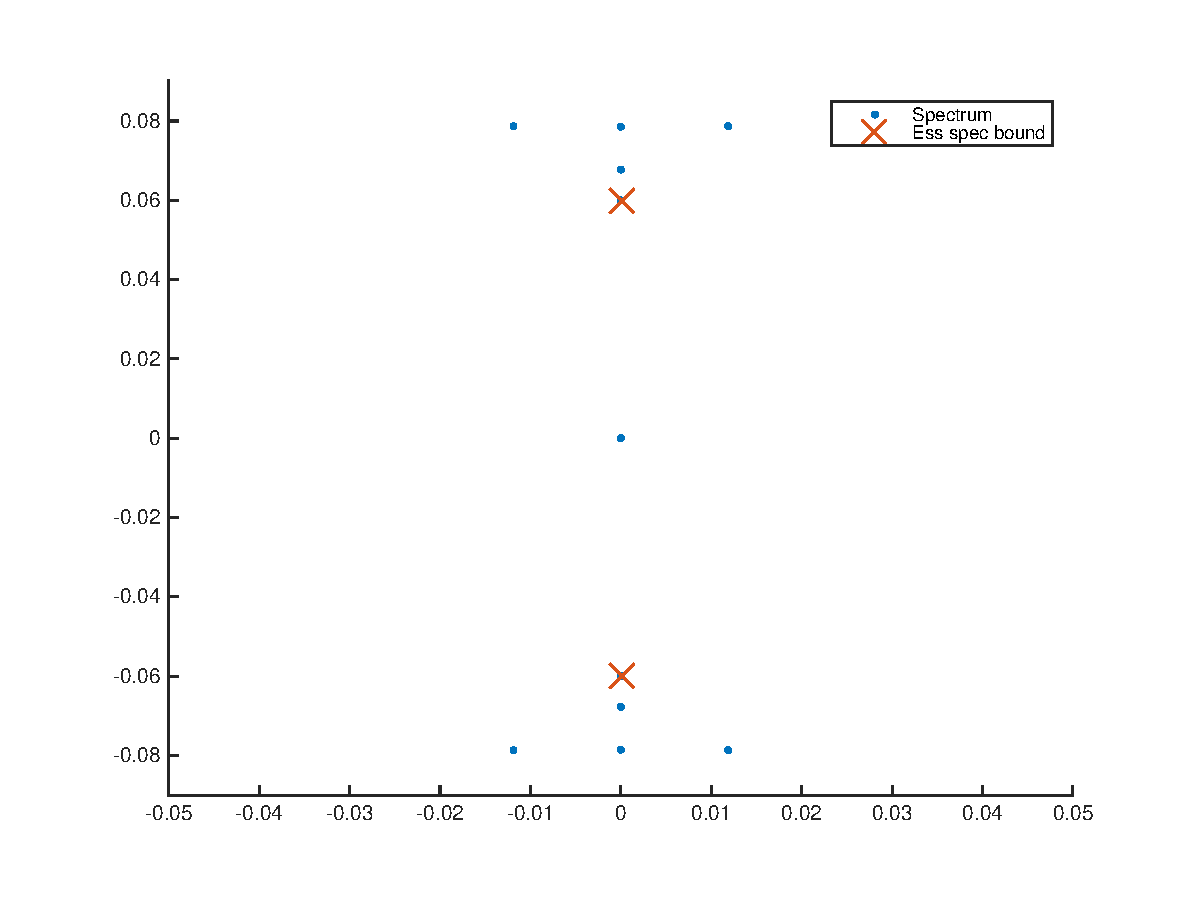
\includegraphics[width=8cm]{spec1354_double2.eps}
\caption{Linearization about Double Pulse 2. Spectrum showing Krein quartet. Finite difference methods, $N = 512$, $c = 1.354$.}
\end{figure}

The final two plots show that the Krein collision occurs between $c = 1.322$ (before collision) and $c = 1.323$ (after collision).

\begin{figure}[H]
\centering
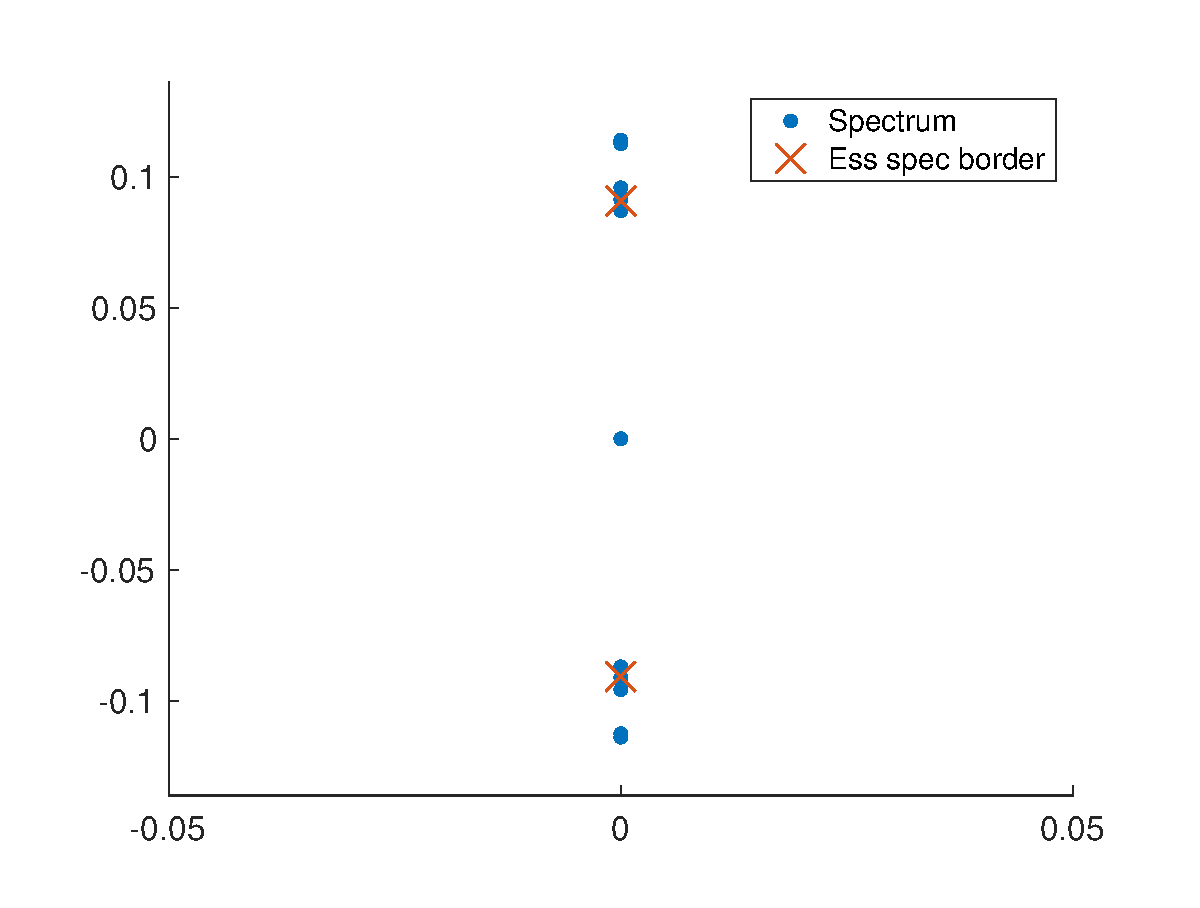
\includegraphics[width=8cm]{spec1322_double2.eps}
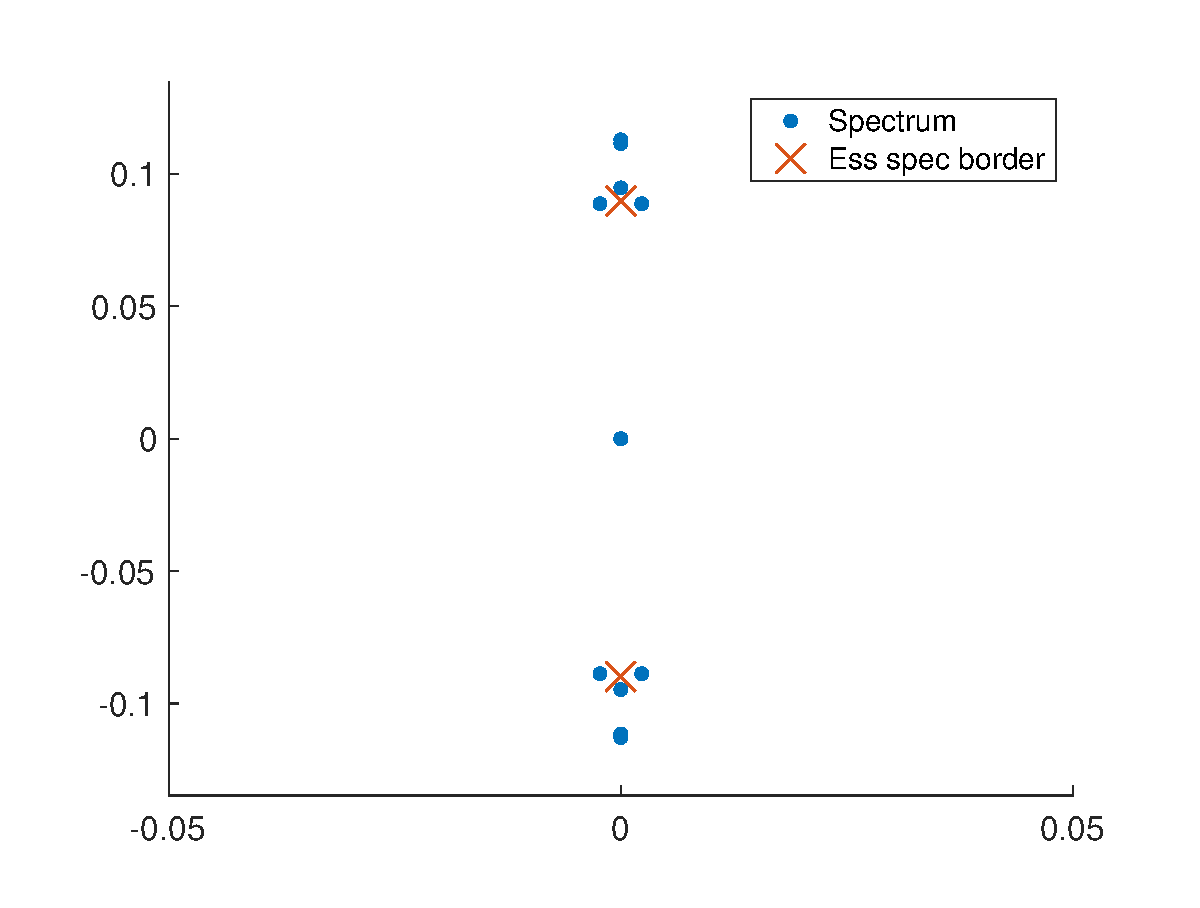
\includegraphics[width=8cm]{spec1323_double2.eps}
\caption{Linearization about Double Pulse 2. Spectrum before Krein collision ($c = 1.322$, left) and after Krein collision ($c = 1.323$, right). Finite difference methods, $N = 512$}
\end{figure}
 
\subsection{Proofs}

\subsubsection{Stability of Primary Pulse}

First, we show stability of the primary pulse $q(x; c)$.

% proposition : primary pulse stability 

\begin{proposition}\label{qstable}
Let $c^2 \in (0, 2)$, and let $q(x; c)$ be the primary pulse solution to \eqref{eqODE}. Then $q(x; c)$ is stable if and only if $d''(c) > 0$, where $d(c)$ is defined in \cite[equation (2.16)]{Grillakis1987}.

\begin{proof}
Let $v = u_t$. Then we can write \eqref{susp3} as the Hamiltonian system

\begin{equation}\label{2dsystem}
\frac{d \textbf{u} }{dt} = J E'(\textbf{u}),
\end{equation}

where $\textbf{u} = \begin{pmatrix}u&v\end{pmatrix}^T$, $J$ is the standard symplectic matrix

\begin{equation*}
J = \begin{pmatrix}0 & 1 \\ -1 & 0 \end{pmatrix}
\end{equation*}

and $E(\textbf{u})$ is the energy

\begin{equation}\label{energy}
E(\textbf{u}) = \int_{-\infty}^\infty \left(\frac{1}{2} v^2 + \frac{1}{2}u_{xx}^2 + e^{u} - u \right)dx
\end{equation}

Equation \eqref{2dsystem} and the energy \eqref{energy} are invariant under the unitary translation group $T(s)$, defined by $T(s)\phi(\cdot) = \phi(\cdot - s)$. \\

We need to verify Assumptions 1, 2, and 3B in \cite{Grillakis1987}. Assumption 1 is the same as Hypothesis \ref{PDEexisthyp}. Assumption 2 follows from the fact that $q(x; c)$ is a bound state, i.e. satisfies in \cite[equation (2.15)]{Grillakis1987}, and from smooth dependence of \eqref{eqODE} on the parameter $c$. Assumption 3B follows from the spectrum of $A_0$. By the Weyl essential spectrum theorem, for $c^2 \in (0, 2)$, the essential spectrum of $A_0(q)$ is 

\begin{equation}\label{A0ess}
\sigma_{\text{ess}}(A_0(q)) = [1 - c^4/4, \infty),
\end{equation}

which is positive and bounded away from 0. By Hypotheses \ref{A0kernel} and \ref{A0neg}, $A_0(q)$ has a simple eigenvalues at 0 and a simple negative eigenvalue. Assumption 3B then follows from the corrected proof of \cite[Lemma 6.2]{Grillakis1987} given in \cite{Grillakis1990}. The result then follows from \cite[Theorem 5.5 and 3]{Grillakis1987}.
\end{proof}
\end{proposition}

\subsubsection{Proof of Theorem \ref{Kreindiag}}

Using Theorem \ref{multiexist}, let $q_n(x; c)$ be an $n-$modal solution to \eqref{eqODE}, and let $\{\nu_1, \dots, \nu_n\}$ be the small eigenvalues of $A_0(q_n)$ with corresponding eigenfunctions $\{ s_1, \dots, s_n \}$. Take the $s_i$ to be orthogonal, and scale them so that

\begin{equation}\label{orthoeigs}
\langle s_i, s_j \rangle = ||q_x(x; c)||^2 \delta_{ij}.
\end{equation}

Define the Krein matrix $K_S(\lambda)$ as on p.4 OF THIS PAPER by 

\begin{equation}
[K_S(\lambda)]_{jk} = 
\langle s_j , P_2(\lambda)s_k\rangle 
- \langle s_j , P_2(\lambda) P_{S^{\perp}} (P_{S^{\perp}} P_2(\lambda)|_{S^{\perp}} )^{-1} P_{S^{\perp}} P_2(\lambda) s_k \rangle.
\end{equation}

Let $\lambda = i z$. Using Lemma 5.6 IN THIS PAPER and \eqref{orthoeigs}, for small $|z|$ the Krein matrix is the $n \times n$ matrix

\begin{equation}\label{Kreinform}
K_S(z) = ||q_x||^2 \text{diag}(\nu_1, \dots, \nu_n) + \overline{z} K_1 
- \overline{z}^2 ( ||q_x||^2 I + K_2) + \mathcal{O}(|z|^3),
\end{equation}

where

\begin{align}
(K_1)_{jk} &= \langle s_j, i A_1 s_k \rangle \label{defK1} \\
(K_2)_{jk} &= \langle P_{S^\perp} A_1 s_j, (P_{S^\perp} A_0(q_n)|_{S^\perp})^{-1} P_{S^\perp} A_1 s_k \rangle \label{defK2}
\end{align}

This is, to leading order, a matrix-valued quadratic polynomial in $z$ (and its complex conjugate). If we take $z \in \R$, the Krein matrix is Hermitian.\\

We now prove Theorem \ref{Kreindiag} in a series of lemmas. 

% lemma : K1 is small

\begin{lemma}\label{K1small}
For the matrix $K_1$ in \eqref{Kreinform}, 

\begin{equation}\label{K1final}
K_1 = \mathcal{O}(e^{-(3 \alpha/2) X_m}).
\end{equation}

\begin{proof}
From \eqref{defK1}, $(K_1)_{jk} = 2 c i \langle s_j, (s_k)_x \rangle$. Using \eqref{sj} from Theorem \ref{multiexist},

\begin{align*}
\langle s_j &, (s_k)_x \rangle 
&= \sum_{m = 1}^{n} d_{jm} d_{km} \langle q^m_x, q^m_{xx} \rangle 
+ \sum_{m \neq l} d_{jm} d_{kl} \langle q^m_x, q^l_{xx} \rangle 
+ \langle s_j, (w_k)_x \rangle 
+ \sum_{m = 1}^{n} d_{km} \langle w_j, q^j_{xx} \rangle.
\end{align*}  

By translation invariance, $\langle q^m_x, q^m_{xx} \rangle = \langle q_x, \partial_x q_x \rangle = 0$ since the operator $\partial_x$ is skew-symmetric. For $m \neq l$, $q^m$ and $q^l$ are exponentially separated by at least $2 X_m$, thus $\langle q^m_x, q^l_{xx} \rangle = \mathcal{O}(e^{-(3 \alpha/2) X_m})$. The last two terms are $\mathcal{O}(e^{-2 \alpha X_m})$ using Holder's inequality and the bound \eqref{sjwbound} from Theorem \ref{multiexist}. Combining these, we obtain \eqref{K1final}.

\end{proof}
\end{lemma}

Using \eqref{sj} from Theorem \eqref{multiexist}, the matrix $K_2$ in \eqref{Kreinform} becomes

\begin{align}\label{K2expansion}
(K_2)_{jk} 
= 4 c^2 \langle &\sum_{l = 1}^{n} d_{jl} q^l_{xx} + (w_j)_x, \\
&\sum_{l = 1}^{n} d_{kl} P_{S^\perp} (P_{S^\perp} A_0(q_n)|_{S^\perp})^{-1} P_{S^\perp} q^l_{xx} + P_{S^\perp} (P_{S^\perp} A_0(q_n)|_{S^\perp})^{-1} P_{S^\perp} (w_k)_x \rangle \nonumber.
\end{align}

Before we can evaluate this, we need to look at the operator $(P_{S^\perp} A_0(q_n)|_{S^\perp})^{-1}$.

% lemma : P_{S^\perp} A_0(q_n) |_{S^\perp} invertible

\begin{lemma}\label{PA0inv}
$P_{S^\perp} A_0(q_n) |_{S^\perp}$ is an invertible linear operator, and its inverse $(P_{S^\perp} A_0(q_n) |_{S^\perp})^{-1}$ is bounded. If $w \in S^\perp$ is smooth, then $y = (P_{S^\perp} A_0(q_n)|_{S^\perp})^{-1} w$ is smooth as well.

\begin{proof}
The operator $P_{S^\perp} A_0(q_n)$ is self-adjoint and is Fredholm with index 0, thus the restriction $P_{S^\perp} A_0(q_n)|_{S^\perp}$ is invertible on $S^\perp$. By \eqref{A0ess}, the essential spectrum of $A_0(q_n)$ is bounded away from 0, and by the definition of $S$ and Theorem \ref{multiexist}, $P_{S^\perp} A_0(q_n)$ has no eigenvalues of magnitude less than $\delta$. Thus, by the resolvent bound for normal operators, $(P_{S^\perp} A_0(q_n)|_{S^\perp})^{-1}$ is a bounded linear operator on $S^\perp$. 
\end{proof}
\end{lemma}

Next, we evaluate the term $(P_{S^\perp} A_0(q_n)|_{S^\perp})^{-1} P_{S^\perp} q^l_{xx}$ from \eqref{K2expansion}.

% lemma : evaluation of (P_{S^\perp} A_0(q_n)|_{S^\perp})^{-1} P_{S^\perp} q^i_{xx}

\begin{lemma}\label{PA0invqxx}

\begin{equation}\label{invqxx}
(P_{S^\perp} A_0(q_n)|_{S^\perp})^{-1} P_{S^\perp} q^l_{xx} = -\frac{1}{2c}P_{S^\perp} q^l_c
+ \mathcal{O}(e^{-2 \alpha X_m}).
\end{equation}

\begin{proof}
By Lemma \ref{PA0inv}, since $P_{S^\perp} q^l_{xx}$ is smooth, the equation

\begin{equation}\label{Linstart}
(P_{S^\perp} A_0(q_n))y = P_{S^\perp} q^l_{xx}
\end{equation}

has a unique smooth solution $y$. Using Lin's method, we will look for a solution to \eqref{Linstart} of the form 

\begin{equation}\label{Linsolform}
y = -\frac{1}{2c} P_{S^\perp} q^l_c + \tilde{w},
\end{equation}

where this ansatz is suggested by 

\begin{equation}\label{uc}
A_0(u_*) \partial_c u^* = -2 c u^*_{xx}.
\end{equation}

Substituting \eqref{Linsolform} into \eqref{Linstart} and simplifying, we are left with

\begin{equation}
A_0(q_n)\tilde{w} + h(x) = 0.
\end{equation}

where $||h(x)|| = \mathcal{O}(e^{-\alpha X_m})$. Since the translates $q^j(x)$ are exponentially separated, for $j = 1, \dots, n$, we can write the operator $A_0(q_n)$ as 

\begin{align}\label{A0expansion} 
A_0(q_n) &= A_0(q^j) + \sum_{k \neq j} (e^{q^k(x)} - 1) + \tilde{h}(x),
\end{align}

where $||\tilde{h}|| = \mathcal{O}(e^{-\alpha X_m})$. Following \cite{Sandstede1998}, we write this as a piecewise first-order system in $n$ pieces, where we use the expansion \eqref{A0expansion} on the $j$th piece. From this, we obtain a unique, piecewise solution 

\begin{align}\label{Linpiecesol}
y_j^\pm &= -\frac{1}{2c} P_{S^\perp} q^l_c + \tilde{w}_j^\pm && j = 1, \dots, n
\end{align}

to \eqref{Linstart}, where we have uniform bound $||\tilde{w}_j^\pm|| = \mathcal{O}(e^{-2 \alpha X_m})$. In general, this solution will have $n - 1$ jumps. In this case, however, it must be smooth since \eqref{Linstart} has a unique, smooth solution $y$ which therefore must be the same as \eqref{Linpiecesol}. 

\end{proof}
\end{lemma}

We prove one more lemma before we evaluate the matrix $K_2$ from \eqref{Kreinform}.

% lemma : orthogonality of coefficients d_{jk}

\begin{lemma}\label{orthogonald}
For the coefficients $d_{jk}$ in \eqref{sj} from Theorem \ref{multiexist}, we have

\begin{equation}\label{dsum}
\sum_{l = 1}^{n} d_{jl} d_{kl} = \delta_{jk} + \mathcal{O}(e^{-(3 \alpha/2) X_m}).
\end{equation}

\begin{proof}
Using the orthogonality relation \eqref{orthoeigs} and \eqref{sj} from Theorem \ref{multiexist},

\begin{align*}
||q_x||^2 \delta_{jk}
&= \sum_{l = 1}^{n} d_{jl} d_{kl} \langle q^l_x, q^l_{x} \rangle 
+ \sum_{m \neq l} d_{jm} d_{kl} \langle q^m_x, q^l_{x} \rangle 
+ \langle s_j, w_k \rangle 
+ \sum_{l = 1}^{n} d_{kl} \langle w_j, q^l_{x} \rangle.
\end{align*}

As in Lemma \ref{K1small}, the second term on the RHS is $\mathcal{O}(e^{-(3 \alpha/2) X_m})$ and the last two terms on the RHS are $\mathcal{O}(e^{-2 \alpha X_m})$. By translation invariance, $\langle q^l_x, q^l_{x} \rangle = \langle q_x, q_{x} \rangle = ||q_x||^2$ for all $l$. Dividing by $||q_x||^2$ gives us \eqref{dsum}.

\end{proof}
\end{lemma}

Finally, we can evaluate the matrix $K_2$ from \eqref{Kreinform}.

% lemma : K2 approx diagonal

\begin{lemma}\label{K2diag}

For the matrix $K_2$ in \eqref{Kreinform}, 

\begin{equation}\label{K2final}
(K_2)_{jk} 
= -2 c \langle q_{xx}, q_c \rangle \delta_{jk} + \mathcal{O}(e^{-(3 \alpha/2) X_m}).
\end{equation}

\begin{proof}
By Lemma \ref{PA0inv}, $(P_{S^\perp} A_0(q_n)|_{S^\perp})^{-1}$ is a bounded linear operator; thus, using the bound \eqref{sjwbound} from Theorem \ref{multiexist}, the final term in \eqref{K2expansion} is $\mathcal{O}(e^{-2 \alpha X_m})$. Using this and substituting \eqref{invqxx} from Lemma \ref{PA0invqxx}, \eqref{K2expansion} becomes

\begin{align*}
(K_2)_{jk} 
&= 4 c^2 \langle \sum_{l = 1}^{n} d_{jl} q^l_{xx} + (w_j)_x, 
-\frac{1}{2c}\sum_{l = 1}^{n} d_{kl} P_{S^\perp} q^l_c + \mathcal{O}(e^{-2 \alpha X_m}) \rangle \\
&= -2 c \left( \sum_{l = 1}^{n} d_{jl} d_{kl} \langle q^l_{xx}, q^l_c \rangle
+ \sum_{m\neq l} d_{jm} d_{kl} \langle q^m_{xx}, q^j_c \rangle
+ \sum_{l=1}^n \langle (w_j)_x, d_{kl} q^l_c \rangle \right) + \mathcal{O}(e^{-2 \alpha X_m}).
\end{align*}

For the first term on the RHS, by translation invariance and Lemma \ref{orthogonald},

\begin{align*}
\sum_{i = 1}^{n} d_{ji} d_{ki} \langle q^i_{xx}, q^i_c \rangle
&= \langle q_{xx}, q_c \rangle \sum_{i = 1}^{n} d_{ji} d_{ki} \\
&= \langle q_{xx}, q_c \rangle \delta_{jk} + \mathcal{O}(e^{-(3 \alpha/2) X_m}).
\end{align*}

Since $q^l_{xx}$ and $q^j_c$ are exponentially separated, the second term on the RHS is $\mathcal{O}(e^{-(3 \alpha/2) X_m})$. Using Holder's inequality and the remainder bound \eqref{sjwbound}, the last term on the RHS is $\mathcal{O}(e^{-2 \alpha X_m})$. Combining these, we obtain \eqref{K2final}.

\end{proof}
\end{lemma}

Using \eqref{K1final} from Lemma \ref{K1small} and \eqref{K2final} from Lemma \eqref{K2diag}, the Krein matrix becomes

\begin{equation}\label{Kreinform2}
K_S(z) = ||q_x||^2 \text{diag}(\nu_1, \dots, \nu_n) 
- ( ||q_x||^2 -2 c \langle q_{xx}, q_c \rangle) I \overline{z}^2  + \mathcal{O}(^{-(3 \alpha/2) X_m}|z| + |z|^3)
\end{equation}

Integrating by parts,

\begin{align*}
K_S(z)
&= ||q_x||^2 \text{diag}(\nu_1, \dots, \nu_n) - \left( \langle q_x, q_x \rangle + c \frac{\partial}{\partial c}\langle q_x, q_x \rangle \right)I\overline{z}^2 + \mathcal{O}(^{-(3 \alpha/2) X_m}|z| + |z|^3)  \\
&= ||q_x||^2 \text{diag}(\nu_1, \dots, \nu_n) -\frac{\partial}{\partial c} \left( c||q_x||^2 \right) I \overline{z}^2  + \mathcal{O}(^{-(3 \alpha/2) X_m}|z| + |z|^3) \\
&= ||q_x||^2 \text{diag}(\nu_1, \dots, \nu_n) + d''(c) I \overline{z}^2  + \mathcal{O}(^{-(3 \alpha/2) X_m}|z| + |z|^3)
\end{align*}

which is \eqref{Kreinapprox} in Theorem \ref{Kreindiag}.

\subsection{Proof of Corollary}

By p.4 OF THIS PAPER, the eigenvalues of \eqref{quadeig} are found by solving $\det K_S(z) = 0$ for $z$. By Theorem \ref{Kreindiag}, we can write the Krein matrix $K_S(z)$ as 

\begin{equation}
K_S(z) = \text{diag}(k_1(z), \dots, k_n(z)) + \mathcal{O}(e^{-\alpha X_m}|z| + |z|^3),
\end{equation}

where

\begin{equation}
k_j(z) = ||q_x||^2 \nu_j + d''(c) \overline{z}^2.
\end{equation}

From \cite{Ipsen2008}, the determinant of $K_S(z)$ is given by

\begin{equation}\label{detK}
\det K_S(z) = \prod_{j = 1}^n (k_j(z) + \tilde{r}_j(z)),
\end{equation}

where $\tilde{r}_j(z) = \mathcal{O}(e^{-(3 \alpha/2) X_m}|z| + |z|^3)$. Thus all that remains is to solve $k_j(z) + \tilde{r}_j(z) = 0$ for $j = 1, \dots, n$.\\

\subsubsection{Neutral stability criterion}

For $j = 1, \dots, n-1$, let $\nu_j < 0$. Since we are looking for purely imaginary eigenvalues, take $z \in \R$. Thus the Krein matrix $K_S(z)$ is Hermitian. By \eqref{detK}, we need to solve

\begin{align}\label{eqforz}
||q_x||^2 \nu_j + d''(c) z^2 + \mathcal{O}(e^{-(3 \alpha/2) X_m}|z| + |z|^3) &= 0 && j = 1, \dots, n-1
\end{align}

The higher order terms in \eqref{eqforz} are real since the Krein matrix is Hermitian. By Hypothesis \ref{dccpos}, $||q_x||^2 \nu_j / d''(c) < 0$ for $j = 1, \dots, n-1$. Let

\begin{equation}\label{epsilon2}
\epsilon_j^2 = -\frac{||q_x||^2 \nu_j}{d''(c)} > 0.
\end{equation}

Then \eqref{eqforz} becomes

\begin{equation}\label{eqforz2}
z^2 - \epsilon_j^2 + \mathcal{O}(e^{-(3 \alpha/2) X_m}|z| + |z|^3) = 0.
\end{equation}

Letting $y = \epsilon_j z$ and noting that $\epsilon_j = \mathcal{O}(e^{-\alpha X_m})$, equation \eqref{eqforz2} becomes

\begin{equation}\label{eqforz3}
y^2 - 1 + \mathcal{O}(\epsilon_j^{1/2 }|y| + \epsilon|y^3|) = 0.
\end{equation}

For sufficiently small $\epsilon_j$, equation \eqref{eqforz3} has two roots at $y = \pm 1 + \mathcal{O}(\epsilon_j^{1/2}$. Thus \eqref{eqforz} has two solutions

\begin{equation}
z_j^\pm = \pm ||q_x|| \sqrt{ -\frac{ \nu_j}{d''(c)} } + \mathcal{O}(e^{-(3 \alpha/2) X_m}),
\end{equation}

where the remainder term is real. Since \eqref{quadeig} has complex-conjugate symmetry of eigenvalues, we conclude that the quadratic eigenvalue problem \eqref{quadeig} has $2n - 2$ eigenvalues which are purely imaginary and are given by \eqref{npulseKreineigs}.

\subsubsection{Instability criterion}

Now suppose $\nu_j > 0$ for one of the small eigenvalues of $A_0(q_n)$. In this case, the Krein matrix is not Hermitian. Define $\epsilon_j^2$ as in \eqref{epsilon2}, but this time $\epsilon_j^2 < 0$. Then $\det K_S(z) = 0$ for 

\begin{equation}
z = -i ||q_x|| \sqrt{ \frac{ \nu_j}{d''(c)} } + \mathcal{O}(e^{-(3 \alpha/2) X_m}).
\end{equation}

Thus \eqref{quadeig} has an eigenvalue at

\begin{equation}
\lambda = ||q_x|| \sqrt{ \frac{ \nu_i}{d''(c)} } + \mathcal{O}(e^{-(3 \alpha/2) X_m}),
\end{equation}

which has positive real part for sufficiently large $X_m$. 


\bibliography{suspension.bib}


\end{document}